\documentclass[11pt,a4paper]{article}

\usepackage{amsmath,amssymb}
\usepackage{geometry}
\usepackage{microtype}
\usepackage{hyperref}
\usepackage{natbib}
\usepackage{setspace}
\usepackage{titlesec}
\usepackage{graphicx}
\usepackage{tikz}
\usetikzlibrary{arrows.meta,positioning,shapes.geometric}
\usepackage{booktabs}
\usepackage{caption}
\usepackage{enumitem}
\usepackage{xcolor}

\geometry{
  top=1.2in, bottom=1.2in,
  left=1.25in, right=1.25in
}

\onehalfspacing

\hypersetup{colorlinks=true,linkcolor=black,citecolor=black,urlcolor=black}

\titleformat{\section}{\large\bfseries}{\thesection.}{0.6em}{}
\titleformat{\subsection}{\normalsize\bfseries}{\thesubsection.}{0.6em}{}
\titlespacing{\section}{0pt}{14pt plus 4pt}{6pt plus 2pt}
\titlespacing{\subsection}{0pt}{10pt plus 2pt}{4pt plus 1pt}

\captionsetup{font=small,labelfont=bf,width=0.88\textwidth}

\newcommand{\simA}{\sim_{\!A}}
\newcommand{\simO}{\sim_{\!O}}
\newcommand{\DA}{D_A(\varphi)}
\newcommand{\RHP}{\mathcal{R}_{H}^{\Pi}}

% ══════════════════════════════════════════════════════════════════════════
\title{\textbf{What Any Mind Must Preserve}\\[4pt]
  {\large Reachability, Representation, and the Missing Criterion\\
  in World-Model Cognition}}

\author{Flyxion\\
  \small Independent Researcher}

\date{}

% ══════════════════════════════════════════════════════════════════════════
\begin{document}
\maketitle

\begin{abstract}
\noindent
Kenneth Craik's 1943 insight---that intelligence requires an internal model
of one's own possible actions, not merely of the world---implies a criterion
that cognitive science has not yet formalised. Any internal model adequate for
planning must preserve the distinctions that determine which futures are
accessible from which states. We call this requirement \emph{admissibility},
and we show that it is a prior condition on intelligent behaviour rather than
one desideratum among many. The central result---the Observational--Interventional
Separation Theorem---establishes that world models learned by predicting
observations cannot guarantee admissibility, because observational equivalence
and interventional equivalence are different mathematical relationships generated
by fundamentally different operations. Three consequences follow. Predictive
world models may silently collapse distinctions that planning requires to be
visible. Safety mechanisms built on inadmissible representations inherit
irrecoverable blind spots. And the degree of failure has a formal measure:
\emph{admissibility distortion}, a quantity that current training objectives
neither measure nor minimise. The framework applies equally to biological and
artificial cognitive systems and connects to affordance theory, Bayesian
inference, and the Conscious Turing Machine. The contribution is not a new
training algorithm but the identification of a criterion that cognitive theory
has so far lacked the tools to name.
\end{abstract}

\noindent\textbf{Keywords:} world models, planning, representation, admissibility,
reachability, cognitive architecture, affordances, AI safety.

\bigskip

% ══════════════════════════════════════════════════════════════════════════
\section{Introduction: What Craik Already Knew}

In 1943, the same year that McCulloch and Pitts published their paper on neural
computation, Kenneth Craik wrote a short book that contains what may be the most
cogent description of what an intelligent mind must do. An organism that carries
``a small-scale model of external reality and its own possible actions within its
head,'' Craik argued, can ``try out various alternatives, conclude which is the
best of them, react to future situations before they arise, utilise the knowledge
of past events in dealing with the present and the future'' \citep{craik1943nature}.

The key phrase is easy to overlook: not merely a model of external reality, but
a model of one's \emph{own possible actions}. A map of the terrain is useful;
a map of the terrain that shows which routes are traversable from where you stand
is qualitatively more useful. Craik was describing the difference between a
world model that represents what \emph{is} and a world model that represents
what \emph{can be reached}.

Contemporary cognitive science has pursued both of these ideals. World model
theories in reinforcement learning, predictive processing, and cognitive
architectures generally aim to build internal representations that are predictively
accurate---that successfully anticipate future observations given current ones.
This is a reasonable goal. But it is, we argue, not the right goal, or not a
sufficient one. A representation can be highly accurate at predicting what will
be seen next while remaining entirely inadequate for deciding what to do next.

The present paper develops this argument formally and identifies what the adequate
criterion looks like. We call it \emph{admissibility}: the property that a
representation preserves the distinctions between states that have different
reachable futures. The criterion is not new in spirit---Gibson's \citeyearpar{gibson1979ecological}
affordance theory expresses something closely related, and Craik's formulation
implies it---but it has not previously been given a mathematical form that would
let us measure whether a given representation satisfies it and how badly it fails
when it does not.

The central result of the paper is that world models learned by predicting
observations \emph{cannot} guarantee admissibility, even in principle. This is
not because predictive learning is inaccurate or underpowered. It is because
observational equivalence and interventional equivalence are different
mathematical objects, and no amount of predictive learning converts one into
the other. This has direct consequences for cognitive science, AI safety, and
the theory of mental representation.

% ══════════════════════════════════════════════════════════════════════════
\section{The Core Distinction: Seeing and Doing}

\subsection{Observational and interventional equivalence}

Suppose an agent occupies state $x$ in some environment. Two kinds of question
can be asked about $x$. The first kind is observational: what will the agent
see if it remains passive and watches? The second kind is interventional: from
$x$, where can the agent go?

These are different questions, and they generate different equivalences between
states. Two states $x_1$ and $x_2$ are \emph{observationally equivalent} if
they produce identical sequences of observations under passive sensing. They
are \emph{interventionally equivalent} if every action available from $x_1$
is available from $x_2$ and leads to the same reachable futures---if they afford
identical possibilities.

The Observational--Interventional Separation Theorem, which we establish formally,
shows that observational equivalence does not imply interventional equivalence.
Two states can look identical to a passive observer while offering radically
different possibilities to an agent that acts. The structural reason is that
observational equivalence is generated by comparing probability distributions
over sensory sequences, while interventional equivalence is generated by comparing
sets of reachable futures. These are different mathematical objects, and no
operation---more data, better models, larger networks---converts one into the other.

\subsection{The cracked beam}

The gap becomes intuitive with an engineering example that serves as the paper's
canonical illustration. Consider two load-bearing beams: one structurally intact,
one with an invisible internal crack. Under passive observation in normal
operating conditions, the two beams look identical---same shape, same colour,
same surface texture, same vibration signature. A passive world model, however
sophisticated, would represent them identically.

But under an intervention---applying a stress load that exceeds the crack
threshold---the two beams have radically different reachable futures. From the
intact beam, the agent can reach futures in which the structure holds. From the
cracked beam, failure states become accessible that are unreachable from the
intact one. The two beams are observationally equivalent but interventionally
inequivalent.

This is not a pathological example. Any latent structural variable that
determines what is possible without affecting what is currently observed
produces the same pattern. A patient's genetic predisposition, a hidden
financial liability, a dormant fault in a software system, a microcrack in an
aircraft component---all are examples of distinctions that passive observation
cannot resolve but that planning critically requires.

\subsection{The inversion problem}

This gap is a geometric form of a deeper epistemological difficulty that
statisticians have long recognised. Classical frequentist methods compute
$P(\text{data} \mid \text{hypothesis})$---the probability of what was seen
given what is assumed---when the scientifically relevant quantity is
$P(\text{hypothesis} \mid \text{data})$---the probability that the hypothesis is
correct given what was seen \citep{jaynes2003probability}. No accumulation of
data computed in the wrong direction resolves this type mismatch.

The observational--interventional gap has the same structure. A world model
trained on $P(\text{observation} \mid \text{state})$ learns to answer
observational questions. The planning-relevant quantity is the reachability
structure---which futures are accessible from which states---and this is not
a datum in the observation distribution. Training on the wrong direction of
conditioning does not converge to the answer to the question not being asked.

% ══════════════════════════════════════════════════════════════════════════
\section{Admissibility: What Planning Requires}

\subsection{Reachability and admissibility equivalence}

Given an agent with a repertoire of actions (a policy class $\Pi$) and a
planning horizon $H$, the \emph{reachability set} of a state $x$ is the
collection of all states the agent can reach from $x$ within $H$ steps under
some available policy. We write this $\mathcal{R}_H^\Pi(x)$.

Two states $x_1$ and $x_2$ are \emph{admissibility-equivalent}---written
$x_1 \simA x_2$---if and only if they have identical reachability sets:
$\mathcal{R}_H^\Pi(x_1) = \mathcal{R}_H^\Pi(x_2)$. The fundamental planning
result (Proposition 1 in the formal treatment) is that if two states are not
admissibility-equivalent, there exists a planning problem---a goal that
specifies which futures are desirable---for which they require different
optimal actions. Any representation that conflates them cannot support that
planning problem, regardless of what else it gets right.

The admissibility relation $\simA$ is the \emph{coarsest} equivalence compatible
with adequate planning. It is maximally permissive: it permits a representation
to collapse any two states whose reachable futures genuinely coincide, and
forbids collapsing any pair whose reachable futures differ. This is the minimal
discrimination a planning-adequate representation must maintain.

This framing connects directly to Gibson's affordance theory. Where Gibson asked
what actions an environment \emph{permits}, admissibility asks which futures an
environment makes \emph{accessible}. Both shift the representational question
from ``what is this?'' to ``what can I do from here?''---and both imply that
a representation organised around the former question may fail the latter.

\subsection{Admissibility distortion}

Given any representation $\varphi$ that maps states to internal codes, the
\emph{admissibility distortion} $D_A(\varphi)$ measures how much the
representation violates admissibility. It is defined as the expected reachability
difference between states that $\varphi$ collapses to the same internal code:

\[
  D_A(\varphi) = \mathbb{E}_{x_1, x_2}\!\left[
    \mathbf{1}_{\varphi(x_1) = \varphi(x_2)}
    \cdot d\!\left(\mathcal{R}_H^\Pi(x_1),\, \mathcal{R}_H^\Pi(x_2)\right)
  \right].
\]

When $D_A(\varphi) = 0$, every pair of states the representation identifies has
identical reachable futures---the representation is admissible. When
$D_A(\varphi) > 0$, the representation has merged states with genuinely different
reachable futures. The magnitude of the distortion reflects the planning cost
of this merging: how different the reachable futures are for the pairs that have
been conflated.

A useful decomposition separates two distinct failure modes. The distortion equals
the probability that two randomly drawn states are collapsed by the representation,
multiplied by the expected reachability difference among collapsed pairs:
\[
  D_A(\varphi) = P(\text{collapsed}) \times \mathbb{E}[\text{reachability difference} \mid \text{collapsed}].
\]
A \emph{broad-compressive} failure occurs when many pairs are collapsed but each
pair's reachable futures are only mildly different. A \emph{catastrophic blind-spot}
failure occurs when very few pairs are collapsed but those particular pairs have
radically different reachable futures---including, potentially, safe versus
dangerous states. These failures call for different responses: the first suggests
reducing overall compression, the second demands targeted auditing of the
representation's most consequential collapses.

\begin{figure}[t]
\centering
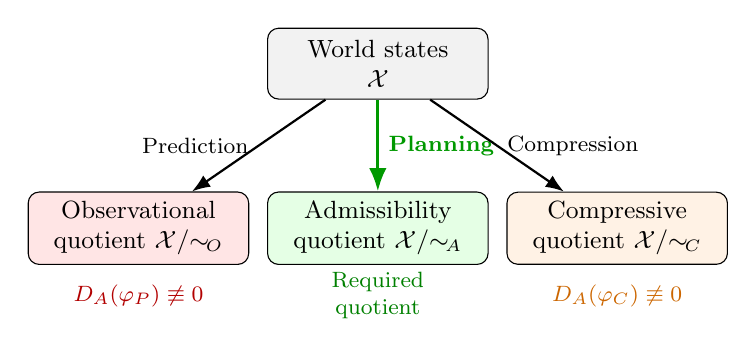
\begin{tikzpicture}[
  box/.style={draw,rounded corners,align=center,minimum width=2.8cm,
              minimum height=0.9cm,font=\small},
  arr/.style={-Latex,thick},
  scale=0.95
]
\node[box,fill=gray!10] (world) at (0,0) {World states\\$\mathcal{X}$};
\node[box,fill=red!10]  (obs)  at (-3.2,-2.2) {Observational\\quotient $\mathcal{X}/{\simO}$};
\node[box,fill=green!10](adm)  at (0,-2.2) {Admissibility\\quotient $\mathcal{X}/{\simA}$};
\node[box,fill=orange!10](comp) at (3.2,-2.2) {Compressive\\quotient $\mathcal{X}/{\sim_{\!C}}$};
\draw[arr] (world) -- (obs)  node[midway,left,font=\footnotesize]{Prediction};
\draw[arr,very thick,green!60!black] (world) -- (adm)
  node[midway,right,font=\footnotesize]{\textbf{Planning}};
\draw[arr] (world) -- (comp) node[midway,right,font=\footnotesize]{Compression};
\node[font=\footnotesize,text=red!70!black] at (-3.2,-3.1)
  {$D_A(\varphi_P) \not\equiv 0$};
\node[font=\footnotesize,text=green!50!black,align=center] at (0,-3.1)
  {Required\\quotient};
\node[font=\footnotesize,text=orange!80!black] at (3.2,-3.1)
  {$D_A(\varphi_C) \not\equiv 0$};
\end{tikzpicture}
\caption{Every representation-learning method proposes a partition of the state
space into equivalence classes. Predictive methods partition by observation
similarity; compressive methods partition by description length. The partition
that planning requires---the admissibility quotient---is generated by a different
criterion: equality of reachable futures. None of the standard objectives
guarantees that their partition coincides with the planning-required one.}
\label{fig:quotients}
\end{figure}

% ══════════════════════════════════════════════════════════════════════════
\section{Why Predictive and Compressive World Models Fall Short}

\subsection{The predictive gap}

Modern world models are trained to predict: given the current state
representation, anticipate future observations. This is the approach taken by
predictive processing theories in cognitive science \citep{clark2013whatever},
by Joint Embedding Predictive Architectures in machine learning, and by virtually
every self-supervised representation-learning system. The resulting representations
are evaluated by how well they predict.

The Separation Theorem shows this is insufficient for planning. Two states that
produce identical observation distributions under passive sensing---and are
therefore treated as equivalent by any predictive objective---may differ in
their reachable futures. A predictive world model that represents them identically
is making a planning error that no amount of predictive accuracy can correct,
because the error is not an inaccuracy about observations but a category mistake
about possibilities.

To use statistical language: predictive learning answers the question
``what will I observe from here?'' Planning requires answering the question
``where can I go from here?'' These questions have different answers and require
different representations. A system optimised for the former is not thereby
optimised for the latter.

\subsection{The compression gap}

Many cognitive theories, and many information-theoretic frameworks for intelligence,
propose that good representations are compressed representations---that a mind
should build the most compact internal model consistent with the data. This
intuition has genuine appeal. Compression generalises; specific memorisation
does not.

But compression creates a structural pressure toward admissibility violation.
Compressing a representation means merging states whose internal codes are
similar, enlarging equivalence classes to reduce description length. The
Monotonicity Theorem shows that this movement is structurally ordered: a better
compressor always has admissibility distortion at least as large as a worse one,
because each compression step merges additional pairs. The increase is exactly
the expected reachability separation of the pairs that the compression step newly
merges---not merely a risk, but an unavoidable cost that compounds with each
compression gain.

This creates a fundamental tension. Compression-efficient representations are
good at ignoring irrelevant detail. But the states most likely to be compressed
away---rare states that deviate from the typical distribution---are exactly the
states most likely to have distinctive reachable futures. The outlier that a
compressor treats as noise is often the outlier that matters most for planning:
the crack in the beam, the anomalous financial signal, the atypical symptom.

\subsection{Compression and Bayesian Occam's razor}

This tension has a mirror image in Bayesian inference. Bayesian model comparison
imposes an automatic Occam's razor: more complex models have their prior
probability diluted across a larger parameter space, and unless that complexity
yields commensurate predictive gain, the marginal likelihood punishes it
\citep{jaynes2003probability}. The Bayesian calculus penalises representations
for exploring unnecessary dimensions.

Admissibility distortion is the dual penalty. Bayesian Occam punishes models
for adding parameters that do not earn their keep by improving prediction.
Admissibility distortion penalises representations for removing distinctions
that planning requires to be preserved. The two mechanisms together bound a
well-posed representational space from opposite sides: unnecessary complexity
is penalised by marginal likelihood dilution; destructive simplicity is penalised
by admissibility distortion.

Current machine learning applies the first penalty (through various regularisers,
cross-validation, and early stopping) but not the second. The admissibility
framework identifies the missing half of the picture.

% ══════════════════════════════════════════════════════════════════════════
\section{Consequences for Safety and Alignment}

\subsection{Irrecoverable blind spots}

One of the most practically significant results concerns the limits of safety
mechanisms built on inadmissible representations. Suppose a world model has
merged two states---one safe, one dangerous---because they produce similar
observations under passive sensing. Any safety classifier, content filter, or
guardrail that operates on the internal representation inherits this blindness.
There is no way for the classifier to distinguish states that the representation
has already declared indistinguishable.

More formally: any computation applied downstream of an inadmissible projection
is bounded in the safety-relevant information it can recover. If the
representation has destroyed the distinction between safe and dangerous states,
no downstream classifier---however complex, however carefully trained---can
recover it. The information-theoretic result (the data-processing inequality)
makes this precise: information about admissibility status cannot increase as
data flows from the projection to the classifier. It can only decrease or
remain constant.

This has a direct implication for AI safety practice. Current approaches often
treat the representation as a given and focus engineering effort on the
classifier---better training data, more careful fine-tuning, more elaborate
safety heads. The admissibility framework shows this is addressing the wrong
stage. If the representation has collapsed a safety-relevant distinction, the
classifier problem is unsolvable. The engineering effort should be directed at
the representation itself.

\subsection{A diagnostic principle}

The admissibility framework provides a practical diagnostic: persistent safety
failure with error rates near chance (50\%) is evidence of representational
inadmissibility rather than classifier inadequacy. A safety system that performs
near-randomly is not failing because its classifier is bad; it is failing because
the representation it operates on has destroyed the relevant information.

Conversely, a witnessed violation is definitive. If two states receive the same
internal representation but are found, by trying different actions, to lead to
different outcomes, this proves that the representation has admissibility
distortion greater than zero. The evidence is one-sided: a witnessed disagreement
proves the representation is inadmissible; absence of witnessed disagreement
proves only that the particular exploration was insufficient to detect
inadmissibility.

\subsection{Safety as a prior condition, not an add-on}

The fundamental implication is that safety mechanisms must be designed with
admissibility in mind at the representation level, not added as a postprocessing
step. This aligns with a broader principle in cognitive science: that the
distinctions a cognitive system draws at the representational level constrain
everything that can be done with those representations downstream. You cannot
reason about distinctions that were collapsed before reasoning began.

% ══════════════════════════════════════════════════════════════════════════
\section{Admissibility as a Universal Cognitive Requirement}

\subsection{Not a criterion for machines only}

The admissibility framework is developed here in the context of artificial
world models, but its logical status is more general. The planning sufficiency
requirement---that any representation adequate for planning must preserve
distinctions between states with different reachable futures---is derived from
what planning requires, not from what machines do. Its premises involve no
assumptions about substrate, architecture, or implementation.

This means the requirement applies to biological cognitive systems with equal
force. A human planner who systematically confuses states with different
reachable futures incurs planning failures by exactly the same mechanism as a
neural network with high admissibility distortion. The errors may look different
in surface form, but the underlying structure is identical: a distinction required
by planning has been collapsed at the representational level, and the planning
failure propagates from that collapse.

\subsection{Adaptability and Scheler's criterion}

This connects the admissibility framework to classical discussions of intelligence.
Max Scheler's criterion for genuine intelligence---the capacity to adapt
immediately and appropriately to entirely novel situations---requires exactly
this: an agent encountering a state it has never seen before must correctly
identify which responses are available from that state. That is a question
about the reachability structure of novel states, and answering it requires
a representation that preserves admissibility. A system with high admissibility
distortion cannot adapt to novel situations in Scheler's sense, regardless of
how accurately it predicts familiar ones.

\subsection{Self-modification and identity}

For agents that undergo developmental change---whether through learning,
biological development, or deliberate self-modification---admissibility extends
to a question about identity across change. An agent remains a coherent
planning agent across a transformation insofar as the transformation preserves
the reachability-relevant distinctions that defined its planning competence.
Transformations that destroy these distinctions are transformations that
undermine the agent's planning identity, not merely its performance.

This provides an admissibility-based reading of proposals for narrative identity
and symbolic self-stabilisation in autonomous AI systems
\citep{graziano2013consciousness}. The question is not whether such systems
maintain a coherent narrative about themselves but whether their self-modifications
preserve admissibility-relevant structure. A coherent narrative built on an
inadmissible self-model will produce coherent-sounding but unreliable planning.

\subsection{Consciousness and world models}

The Conscious Turing Machine \citep{blum2022conscious} provides an illuminating
case study. In that architecture, a global broadcast mechanism selects a
``chunk''---a compressed representation of the agent's current situation---and
distributes it to all cognitive processors simultaneously. The chunk is the
pivot around which all downstream processing turns.

If the chunk representation is inadmissible---if the chunk selection process
collapses states with genuinely different reachable futures into the same
broadcast---then every downstream processor will reason from a representation
that has already made a planning error. The resulting behaviour will be
internally coherent (all processors received the same chunk) but planning-deficient
(the chunk did not preserve the distinctions that planning requires).

Francisco Varela's definition of first-person experience as the ``lived
experience associated with cognitive and mental events'' with a ``subjective
side'' \citep{varela1999first} implies that genuine experience involves genuine
engagement with one's situation. If the represented situation is inadmissibly
distorted---if what is experienced as ``the possibilities open to me'' does not
correspond to the actual reachable futures---then experience is systematically
misleading in a way that goes beyond ordinary error. Admissibility is not
sufficient for consciousness, but it appears to be a necessary condition for
the kind of reliable, world-engaging experience that cognitive theories target.

% ══════════════════════════════════════════════════════════════════════════
\section{What an Admissible World Model Would Look Like}

\subsection{The representational target}

The admissibility framework does not prescribe a specific architecture. It
identifies a criterion: a representation is adequate for planning if and only
if it never collapses two states with different reachable futures. This criterion
can in principle be approached by many different architectural choices.

What the framework rules out---or more precisely, identifies as insufficient---is
the strategy of learning a representation through passive observation and hoping
that planning-relevant distinctions are preserved incidentally. The Separation
Theorem shows this hope cannot be vindicated in general. A representation that
is genuinely aimed at planning adequacy must either incorporate admissibility
as an explicit objective or operate in a regime where observational and
interventional equivalence happen to coincide (which is an additional structural
property that must be independently verified, not assumed).

\subsection{How to detect failures}

The most practically useful result of the framework is not the impossibility
theorem but the diagnostic it enables. Given a trained world model, admissibility
violations can be detected by active exploration: take two states that the
model represents identically, try available actions from each, and observe
whether their outcomes diverge. If outcomes diverge, the representation has
admissibility distortion greater than zero. The violation has been witnessed.

This is a Popperian diagnostic: it can falsify a representation's admissibility
but cannot certify it. Failure to find a violation with a given set of exploratory
policies proves only that those particular policies were insufficient witnesses,
not that no violations exist. But witnessed violations are definitive---they
provide principled grounds to distrust a representation's adequacy for planning,
independently of its predictive accuracy.

\subsection{The compression--admissibility tradeoff}

A natural formulation of admissibility-aware representation learning treats the
problem as a constrained optimisation: find the most compact representation
subject to keeping admissibility distortion below a tolerable threshold. The
Lagrangian relaxation of this problem adds an admissibility penalty to the
compression objective:
\[
  \min_\varphi \;\big[\text{description length} + \lambda \cdot D_A(\varphi)\big].
\]
At $\lambda = 0$ this reduces to ordinary compression with no admissibility
constraint; as $\lambda \to \infty$ it forces the representation to be
admissible at the cost of reduced compression. The Lagrange multiplier $\lambda$
controls the compression--admissibility tradeoff, and the rate at which the
optimal objective changes with $\lambda$ equals the current admissibility
distortion---a fact that provides one diagnostic handle on the tradeoff.

This formulation mirrors the Bayesian information bottleneck
\citep{jaynes2003probability,tishby1999information}: compress maximally while
retaining the relevant information. The novelty is identifying planning-relevant
information as reachability structure rather than prediction targets.

% ══════════════════════════════════════════════════════════════════════════
\section{Discussion}

\subsection{What admissibility does and does not claim}

The admissibility framework makes a necessary-condition claim, not a
sufficiency claim. A representation with zero admissibility distortion is
adequate for planning in the sense that it does not err by collapsing
planning-relevant distinctions. It is not thereby adequate for understanding,
consciousness, creativity, or the full range of cognitive competences that
interest cognitive science. Those phenomena may require much more than
admissibility.

What the framework claims is narrower and, for that reason, more defensible:
inadmissibility is sufficient for planning failure, and admissibility is necessary
for adequate planning. This is a genuine contribution to cognitive theory
because it identifies a concrete structural property that any cognitive or
computational system capable of planning must possess, and provides a formal
criterion for whether that property holds.

\subsection{Limitations and future directions}

The framework as presented assumes a fixed state space, a fixed repertoire
of available actions, and a fixed planning horizon. Real cognitive systems
are not like this: they learn new actions, discover new state descriptions,
and vary their planning horizons with task demands. Extending admissibility
to settings where the state space itself evolves is an important open problem.
A system that continuously expands its behavioural repertoire must continuously
revise its admissibility relation, and preserving coherent planning identity
across such revisions is a form of the meta-admissibility problem discussed
in the mathematical treatment.

The framework also focuses on reachability in the sense of accessible outcomes.
Planning under partial observability, where the agent does not directly observe
the full state, requires a version of admissibility defined over belief states
rather than world states. Information-state representations in partially
observable environments \citep{kaelbling1998planning} already address part
of this problem; admissibility provides a further constraint on what such
representations must preserve.

\subsection{A missing quantity found}

The contribution of this paper is the identification of admissibility distortion
as a quantity that cognitive science and AI have so far lacked the means to
name. Cognitive theories of world models specify that internal representations
must be accurate, coherent, and generalisable. They do not, as yet, specify
that internal representations must be admissibility-preserving---even though
Craik's original formulation implies it, Gibson's affordance theory implies it,
and the formal results show it follows necessarily from what planning requires.

Admissibility distortion joins the company of other quantities that became
scientifically productive once named: entropy, mutual information, Kolmogorov
complexity, Wasserstein distance. These quantities did not solve the problems
they named, but they organised those problems and pointed toward solutions. The
same is true of admissibility distortion: naming what world models fail to
preserve is the first step toward preserving it.

% ══════════════════════════════════════════════════════════════════════════
\section{Conclusion}

Kenneth Craik's insight---that intelligence requires a model of one's own
possible actions, not merely of the world---implies a constraint on mental
representation that cognitive science has not yet formalised. That constraint
is admissibility: the requirement that a world model preserve the distinctions
between states that have different reachable futures.

We have shown that predictive world models cannot guarantee admissibility,
because observational equivalence and interventional equivalence are
fundamentally different relationships. We have given this failure a formal
measure---admissibility distortion---and derived its properties. We have shown
that safety mechanisms built on inadmissible representations inherit
irrecoverable blind spots. And we have argued that the requirement is universal:
biological and artificial cognitive systems alike must satisfy it to plan
reliably.

The result is not a finished engineering solution but a diagnosis and a target.
Current world model research has been optimising the wrong quantity---predictive
accuracy rather than admissibility preservation---not because predictive accuracy
is unimportant but because the right quantity had not been identified. It now has
a name.

\bigskip
\noindent\textbf{Acknowledgements.} The author has no institutional affiliation
and no conflicts of interest to declare.

% ══════════════════════════════════════════════════════════════════════════
\begin{thebibliography}{99}

\bibitem[Blum \& Blum(2022)]{blum2022conscious}
Blum, L., \& Blum, M. (2022).
A theoretical computer science perspective on consciousness.
\textit{Journal of Artificial Intelligence and Consciousness}, 9(1), 1--42.

\bibitem[Clark(2013)]{clark2013whatever}
Clark, A. (2013).
Whatever next? Predictive brains, situated agents, and the future of cognitive
science.
\textit{Behavioral and Brain Sciences}, 36(3), 181--204.

\bibitem[Cover \& Thomas(2006)]{cover2006elements}
Cover, T.~M., \& Thomas, J.~A. (2006).
\textit{Elements of Information Theory}, 2nd ed.
Wiley.

\bibitem[Craik(1943)]{craik1943nature}
Craik, K.~J.~W. (1943).
\textit{The Nature of Explanation}.
Cambridge University Press.

\bibitem[Ferns et al.(2004)]{ferns2004metrics}
Ferns, N., Panangaden, P., \& Precup, D. (2004).
Metrics for finite Markov decision processes.
\textit{Proceedings of UAI}, 162--169.

\bibitem[Gibson(1979)]{gibson1979ecological}
Gibson, J.~J. (1979).
\textit{The Ecological Approach to Visual Perception}.
Houghton Mifflin.

\bibitem[Graziano(2013)]{graziano2013consciousness}
Graziano, M.~S.~A. (2013).
\textit{Consciousness and the Social Brain}.
Oxford University Press.

\bibitem[Gupta \& Pruthi(2025)]{gupta2025world}
Gupta, T., \& Pruthi, D. (2025).
Beyond world models: Rethinking understanding in AI models.
\textit{arXiv}:2511.12239.

\bibitem[Jaynes(2003)]{jaynes2003probability}
Jaynes, E.~T. (2003).
\textit{Probability Theory: The Logic of Science}.
Cambridge University Press.

\bibitem[Kaelbling et al.(1998)]{kaelbling1998planning}
Kaelbling, L.~P., Littman, M.~L., \& Cassandra, A.~R. (1998).
Planning and acting in partially observable stochastic domains.
\textit{Artificial Intelligence}, 101(1--2), 99--134.

\bibitem[Knuth \& Skilling(2012)]{knuth2012foundations}
Knuth, K.~H., \& Skilling, J. (2012).
Foundations of inference.
\textit{Axioms}, 1(1), 38--73.

\bibitem[Li et al.(2006)]{li2006towards}
Li, L., Walsh, T.~J., \& Littman, M.~L. (2006).
Towards a unified theory of state abstraction for MDPs.
\textit{ISAIM}, 531--539.

\bibitem[Pearl(2009)]{pearl2009causality}
Pearl, J. (2009).
\textit{Causality: Models, Reasoning, and Inference}, 2nd ed.
Cambridge University Press.

\bibitem[Poincar\'e(1914)]{poincare1914}
Poincar\'e, H. (1914).
\textit{Science and Method}.
Thomas Nelson.

\bibitem[Tishby et al.(1999)]{tishby1999information}
Tishby, N., Pereira, F.~C., \& Bialek, W. (1999).
The information bottleneck method.
\textit{Proceedings of the 37th Allerton Conference}, 368--377.

\bibitem[Varela et al.(1999)]{varela1999first}
Varela, F.~J., Shear, J., et al.\ (Eds.) (1999).
\textit{The View from Within: First-Person Approaches to the Study
of Consciousness}.
Imprint Academic.

\bibitem[Wilson(1975)]{wilson1975renormalization}
Wilson, K.~G. (1975).
The renormalization group: Critical phenomena and the Kondo problem.
\textit{Reviews of Modern Physics}, 47(4), 773--840.

\end{thebibliography}

\end{document}
